\section{Ultrasonic Transducers}

The ultrasonic transducer chosen for this project is the CUSA-T80-15-2400-TH. It has an operating frequency of $40kHz$ and tolerates a supply voltage up to $80V$.\cite{cui_devices_cusa-t80-15-2400-th_2020}\newpage
\noindent One module uses $19$ transducers which are connected in parallel as shown in figure \ref{fig:pcb:transducer_circuit}. In order to create the aspired beamforming effect the transducers are evenly distributed on the pcb (figure \ref{fig:pcb:front}).
%
\begin{figure}
  \centering
  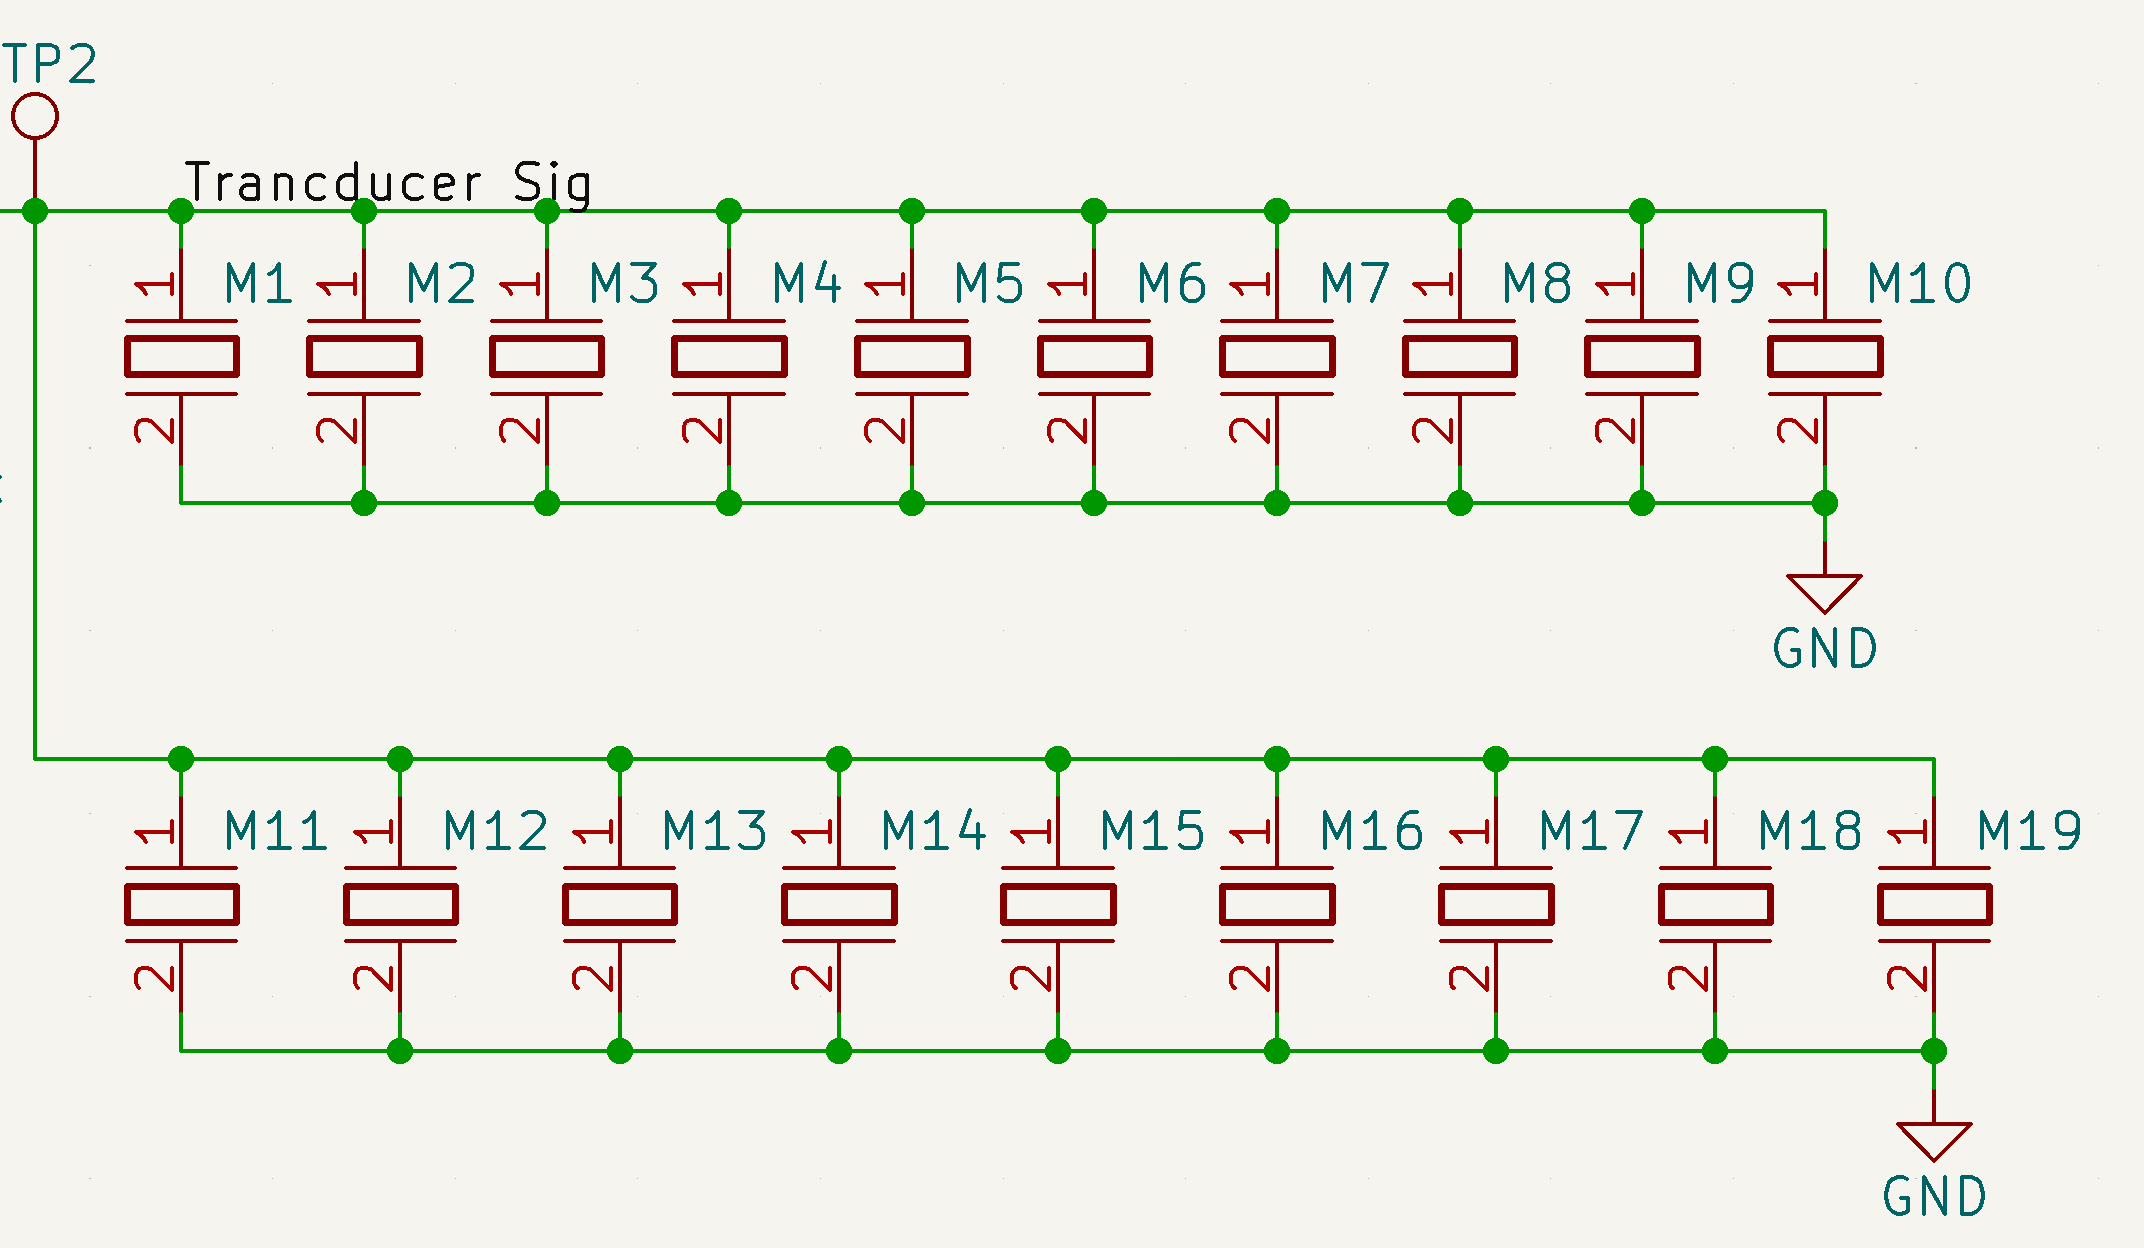
\includegraphics[height=\mediumheight]{src/assets/pictures/circuit/transducer_circuit.png}
  \caption{Transducer circuit design}\label{fig:pcb:transducer_circuit}
\end{figure}